%----------------------------------------------------------------------------------------
%	PACKAGES AND OTHER DOCUMENT CONFIGURATIONS
%----------------------------------------------------------------------------------------

\documentclass{article}

\usepackage{fancyhdr} % Required for custom headers
\usepackage{lastpage} % Required to determine the last page for the footer
\usepackage{extramarks} % Required for headers and footers
\usepackage{graphicx} % Required to insert images
\usepackage{pdflscape} % Allow us to make certain pages in landscape orientation
\usepackage{amsmath} % Allow multiple line equations
\usepackage{amssymb}
\usepackage{scrextend}
\usepackage{xcolor}
\usepackage{listings}

\definecolor{mGreen}{rgb}{0,0.6,0}
\definecolor{mGray}{rgb}{0.5,0.5,0.5}
\definecolor{mPurple}{rgb}{0.58,0,0.82}
\definecolor{backgroundColour}{rgb}{0.95,0.95,0.92}

\lstdefinestyle{CStyle}{
    backgroundcolor=\color{backgroundColour},   
    commentstyle=\color{mGreen},
    keywordstyle=\color{magenta},
    numberstyle=\tiny\color{mGray},
    stringstyle=\color{mPurple},
    basicstyle=\footnotesize,
    breakatwhitespace=false,         
    breaklines=true,                 
    captionpos=b,                    
    keepspaces=true,                 
    numbers=none,                   
    numbersep=5pt,                  
    showspaces=false,                
    showstringspaces=false,
    showtabs=false,                  
    tabsize=2,
    language=C
}

\lstdefinestyle{CStyleInline}{
    backgroundcolor=\color{white},   
    commentstyle=\color{mGreen},
    keywordstyle=\color{magenta},
    numberstyle=\tiny\color{mGray},
    stringstyle=\color{mPurple},
    basicstyle=\footnotesize,
    breakatwhitespace=false,         
    breaklines=true,                 
    captionpos=b,                    
    keepspaces=true,                 
    numbers=none,                   
    numbersep=5pt,                  
    showspaces=false,                
    showstringspaces=false,
    showtabs=false,                  
    tabsize=2,
    language=C
}

% Margins
\topmargin=-0.45in
\evensidemargin=0in
\oddsidemargin=0in
\textwidth=6.5in
\textheight=9.0in
\headsep=0.25in 

\linespread{1.1} % Line spacing

% Set up the header and footer
\pagestyle{fancy}
\chead{} % Top center header
\lhead{\Title}
\rhead{Pedro Alves (9424342)} % Top right header
\lfoot{} % Bottom left footer
\cfoot{} % Bottom center footer
\rfoot{Page\ \thepage\ of\ \pageref{LastPage}} % Bottom right footer
\renewcommand\headrulewidth{0.4pt} % Size of the header rule
\renewcommand\footrulewidth{0.4pt} % Size of the footer rule

\setlength\parindent{0pt} % Removes all indentation from paragraphs

%----------------------------------------------------------------------------------------
%	DOCUMENT STRUCTURE COMMANDS
%----------------------------------------------------------------------------------------

\setcounter{secnumdepth}{0} % Removes default section numbers
   
%----------------------------------------------------------------------------------------
%	NAME AND CLASS SECTION
%----------------------------------------------------------------------------------------

\newcommand{\Title}{Assignment 2} % Assignment title
\newcommand{\DueDate}{21 April 2018} % Due date
\newcommand{\Class}{CAB202 - Microprocessors and Digital Systems} % Course/class
\newcommand{\AuthorName}{Pedro Alves (n9424342)}

%----------------------------------------------------------------------------------------
%	TITLE PAGE
%----------------------------------------------------------------------------------------

\title{
\vspace{2in}
\textmd{\huge\textbf{\Class}}\\
\textmd{{\Title}}\\
\vspace{3in}
\textmd{{\AuthorName}}\\
}

%----------------------------------------------------------------------------------------

\begin{document}

\maketitle
\clearpage

%----------------------------------------------------------------------------------------
%	EXECUTIVE SUMMARY
%----------------------------------------------------------------------------------------
\section*{Executive Summary}

\clearpage

%----------------------------------------------------------------------------------------
%	TABLE OF CONTENTS
%----------------------------------------------------------------------------------------

%\setcounter{tocdepth}{1} % Uncomment this line if you don't want subsections listed in the ToC

\newpage
\tableofcontents
\newpage

%----------------------------------------------------------------------------------------
%	INSTRUCTIONS
%----------------------------------------------------------------------------------------
\section{Instructions}
\begin{enumerate}
	\item Attempt to drive as far as possible without running out of fuel or HP. You win by crossing the finish line
	\item HP is lost by hitting obstacles
	\item Immediate death if a fuel station is hit
	\item To refuel, hold break while immediately next to a fuel station. The car will be pitted automatically if travelling under the pit limit (speed less than 3) with the breaks held
\end{enumerate}
\subsection*{General}
\begin{center}
\begin{tabular}{ c c c }
Function 	& Input 		& Key \\ \hline
Decrease contrast	& Scroll right up 	& Pot1	\\
Increase constrast 	& Scroll right down	& Pot1	\\
\end{tabular}
\end{center}

\subsection*{Splash Screen}
\begin{center}
\begin{tabular}{ c c c }
 Function 	& Input 		& Key \\ \hline
 Play game 	& Left button 	& SW2 \\  
 Play gmae 	& Right button 	& SW3    
\end{tabular}
\end{center}

\subsection*{Game}
\begin{center}
\begin{tabular}{ c c c }
 Function 	& Input 		& Key \\ \hline
 Move left	& Joystick left	& SW1	\\
 Move right	& Joystick right	& SW1	\\
 Pause	& Joystick center 	& SW1	\\
 Accelerate	& Button right	& SW3	\\ 
 Decelerate	& Button left		& SW2	\\
 Limit speed	&			&		\\
 Increase Limit & Left scroll up 	& Pot0	\\
 Decrease Limit & Left scroll down & Pot0
\end{tabular}
\end{center}

\subsection*{Game Paused}
\begin{center}
\begin{tabular}{ c c c }
Function 	& Input 		& Key \\ \hline
Unpause	& Joystick center 	& SW1	\\
Save game	& Joystick up 	& SW1	\\
Load game 	& Joystick down	& SW1	\\
\end{tabular}
\end{center}

\subsection*{Game Over screen}
\begin{center}
\begin{tabular}{ c c c }
Function 	& Input 		& Key \\ \hline
Play again	& Button right	& SW3	\\
Splash screen& Button left 	& SW2 	\\
Load game 	& Joystick down 	& SW1	\\
\end{tabular}
\end{center}

\clearpage

%----------------------------------------------------------------------------------------
%	PROGRAM OVERVIEW
%----------------------------------------------------------------------------------------
\section{Program Overview}
\emph{Zombie Race} is a top-down racing game where the player attempts to drive as far as possible without running out of fuel or colliding with an obstacle. The implementation of this game has been split into several stages that are explained in the later sections. 
\newline
\newline
The basic architecture of the program is that of a state machine. The states for this program are the different screens which the user can see and each provides different functionalities that will be further explored in their specific sections. 
\begin{lstlisting}[style=CStyle]
	// Lines 
	enum GameScreens {
		START_SCREEN,
		GAME_SCREEN,
		GAMEOVER_SCREEN,
	} game_screen;
\end{lstlisting}
After initial setup is complete, the program enters an infinite loop that runs at a rate of about 60 times per second. Inside the loop are two functions, \emph{update()} and \emph{draw()}.
\begin{lstlisting}[style=CStyle]
	// Lines 
	void update(void)
\end{lstlisting}
This function calls the specific update function for the current state the game is in. It will also handle input from \emph{Pot0} that controls the current contrast level of the LCD screen and will perform some operations to allow other functions to use edge detection of the teensy's inputs (ie. only update when clicked). 
\begin{lstlisting}[style=CStyle]
	// Lines 
	void draw(void)
\end{lstlisting}
Will call the draw function of the current state the program is in. Draw function do not change any variables and serve only to write to the LCD through the use of a buffer or directly. Direct draw calls to the LCD will be further explored in the section \emph{Direct screen update}. 
\begin{lstlisting}[style=CStyle]
	// Lines 
	void teensy_setup(void)
\end{lstlisting}
Performs all preliminary calls to setup registers and variables that will be used throughout the program. Will set the clock speed to 8 MHz and the initial LCD contrast to default. The other calls that occur in this functions will be explored in the later sections as they become relevant. 
\clearpage

%----------------------------------------------------------------------------------------
%	TESTING PROCEDURES
%----------------------------------------------------------------------------------------
\section{Testing Procedures}
Due to difficulties with capturing the state of the game directly from the screen of the Teensy, a USB bi-directional communication was set-up between the Teensy and a server. The current value of variables can then be sent as messages to the server in order to assist with debugging, testing and saving/loading. 
\newline
\newline
In order to run the server, enter the command through the Cygwin terminal: \emph{./server /dev/ttyS2} where \emph{ttyS2} is the device name of the Teensy. If this doesn't match, use the command \emph{ls /dev} to find the name for the Teensy currently connected. 
\newline
\newline
The functions used to achieve USB communications will be explored in the section \emph{Bidirectional serial communication and access to file system}. 
\newline
\newline
Testing was accomplished by sending the current state of selected variables via the function \emph{usb\_send\_message()}. Multiple states were then compared to verify if the actual outcome matches the expected outcome.
\newline
\newline
Figure \ref{test_debug} shows the result in the server program when the following command is run
\begin{lstlisting}[style=CStyle]
	usb_send_message(DEBUG, 4, buf, 100, "Timestep: %.3f\nCondition: %d\nFuel: %d\nDistance:  %d\n%d\n", elapsed_time(game_timer_counter), condition, fuel, distance, 0);
\end{lstlisting}
\begin{figure}[!ht]
	\begin{center}
	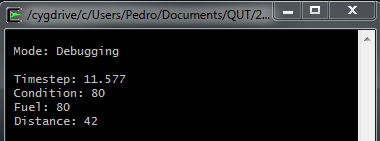
\includegraphics[width=0.8\paperwidth]{images/testing_debug}
	\caption{Screenshot of the server program when a debug command is sent with the current variable states}
	\label{test_debug} 
	\end{center}
\end{figure}
To improve readability of the test plan in the later sections, the information received from the server will be scribed into a table format. Under each teest case, the lines that contain the pieces of code that need to be uncommented to replicate the test are included. 
\newline
\newline
Testing was done by using a srand seed of 100 in order to allow reproduction later of the same tests. 
\clearpage

%----------------------------------------------------------------------------------------
%	SPLASH SCREEN
%----------------------------------------------------------------------------------------
\section{Splash Screen}
The splash screen is the first screen shown when the game is started. After the game is over, the player also has a choice to return to the splash screen. It will display the name of the game and name of the author while waiting for the user to choose to continue playing. The user can choose to start the game by pressing the SW2 or SW3 buttons.

\subsection*{Globals}
\begin{lstlisting}[style=CStyle]
	// Line 
	GameScreens START_SCREEN;
\end{lstlisting}
The value \emph{START\_SCREEN} from the \emph{GameScreens} enum is associated with the splash screen. For more info on the \emph{GameScreens} enum global, see \emph{Program Overview}. 
\begin{lstlisting}[style=CStyle]
	// Line 
	uint8_t button_left_state;
	// Line
	uint8_t button_right_state;
\end{lstlisting}
The current states of the SW2 (left) and SW3 (right) buttons (for more info see \emph{Debouncing}). A state of 1 means the button is pressed. The splash screen will change to the game screen as soon as any of these two variables have a value of 1. 
\newline

\subsection*{Functions}
\begin{lstlisting}[style=CStyle]
	// Lines 
	void start_screen_update(void)
\end{lstlisting}
The update function associated with the splash screen that will be called every tick of the game loop. Will check if SW2 or SW3 have been pressed and call \emph{change\_screen(GAME\_SCREEN)} if true.
\begin{lstlisting}[style=CStyle]
	// Lines 
	void start_screen_draw(void)
\end{lstlisting}
Will call \emph{draw\_string()} to print the name of the game, name of the author and student number to the teensy LCD.  
\newline

\subsection*{Testing}
The following test cases need to pass for this section's tests: 
\begin{itemize}
	\item Game starts when SW2 is pressed
	\item Game starts when SW3 is pressed
\end{itemize}
\subsubsection*{Test Case: Game starts when SW2 or SW3 is pressed}
Lines 457 and 471. A dash in the timestep means that digit was changing rapidly in the server's window.
\begin{center}
\begin{tabular}{ c c c c c }
Timestep	& button\_left\_state	& button\_right\_state	&  game\_screen		& Test result		\\ \hline
0.00-		& 0				& 0				& 1 (START\_SCREEN)	& Pass		\\
0.006		& 0				& 1				& 2 (GAME\_SCREEN)	& Pass		\\
0.00- 		& 0				& 0 				& 1 (START\_SCREEN)	& Pass		\\
0.004		& 1				& 0				& 2 (GAME\_SCREEN)	& Pass		\\ \hline
\end{tabular}
\end{center}
\clearpage

%----------------------------------------------------------------------------------------
%	DASHBOARD
%----------------------------------------------------------------------------------------
\section{Dashboard}
A sub-window in the LCD which displays stats about the player car such as the condition, fuel and speed. A border separates the player from the dashboard area and the player's car is unable to physically move past it (for more info on this, refer to the section \emph{Collision}). It will also display the character 'R' to notify the player that the car is currently refuelling. 

\subsection*{Globals}
\begin{lstlisting}[style=CStyle]
	// Lines 110 - 112
	uint8_t condition;
	uint8_t fuel;
	double speed;
\end{lstlisting}
The variables that hold information about the car. They are modified by other functions thus the dashboard only reads their current values.
\begin{lstlisting}[style=CStyle]
	// Line
	bool refuelling;
\end{lstlisting}
Used to check if the car is currently refuelling. \emph{dashboard\_draw()} will check this and draw the character 'R' if true.
\begin{lstlisting}[style=CStyle]
	// Line
	#define DASHBOARD_BORDER_X  26
\end{lstlisting}
The right-most x coordinate of the dashboard. The border is drawn at this line
\newline

\subsection*{Functions}
\begin{lstlisting}[style=CStyle]
	// Lines 
	void dashboard_draw(void);
\end{lstlisting}
Called in the draw function of the game screen. Will draw the line separating the dashboard from the rest of the game screen then will call the \emph{draw\_string()} and \emph{draw\_formatted()} functions in other to display the current game information. If the player is currently refuelling, will display the character 'R' at the bottom. 
\newline

\subsection*{Testing}
Testing for this section is a mixture of server and visual analysis. The current values to be displayed on the dashboard are sent to the server and visual analysis of the Teensy's LCD screen will determine if the test has passed.
\subsubsection*{Test Case: Values are correctly displayed}
\begin{center}
\begin{tabular}{ c c c c c }
Timestep	& Condition	& Fuel		& Speed	& Test result	\\ \hline
0.102		& 100		& 100		& 10		& Pass	\\
10.289	& 80		& 78		& 6		& Pass	\\ 
21.383	& 40		& 86		& 1		& Pass	\\ \hline
\end{tabular}
\end{center}
All the tests passing mean that the expected values (the ones in the table and shown in the server) match the values seen in the dashboard.

\clearpage

%----------------------------------------------------------------------------------------
%	PAUSED VIEW
%----------------------------------------------------------------------------------------
\section{Paused View}
The user can pause the current game by pressing the center joystick command (SW1). This is only possible when the game state is \emph{GAME\_SCREEN}. The paused screen will display extra information such as the total distance travelled by the car and the elapsed time since the start of the game. While the rest of the game view will be behind the paused view, the player's car can still be visible in order to facilitate the regain of control when unpaused. The time only increases when the game is being played, therefore the counter associated with the current game time must be paused when the paused view is active.

\subsection*{Globals}
\begin{lstlisting}[style=CStyle]
	// Line
	uint8_t distance;
	// Line
	uint16_t game_timer_counter;
\end{lstlisting}
The information that is displayed in the Paused View. These variables are modifed in other sections and Paused View only reads their current value.
\begin{lstlisting}[style=CStyle]
	// Line
	uint8_t game_paused;
\end{lstlisting}
Determines if the game's Paused View should be active or not. Modified by the centre Joystick.
\begin{lstlisting}[style=CStyle]
	// Line
	double time_paused;
\end{lstlisting}
The return value from \lstinline{elapsed_time(game_timer_counter)}. The value is set when the game is paused to avoid the thrid decimal point of the time value fluctuating widly due to floating point precision.
\begin{lstlisting}[style=CStyle]
	// Lines
	uint8_t stick_centre_state;
	uint8_t prev_stick_centre_state;
\end{lstlisting}
\emph{game\_paused} is only toggled when the middle joystick is clicked and just held. This avoid the game pausing and un-pausing multiple times when the user only intended to pause or unpause once with one click. 
\newline

\subsection*{Functions}
\begin{lstlisting}[style=CStyle]
	// Lines
	double elapsed_time(uint16_t timer_counter)
\end{lstlisting}
Used to get the time since the game started in seconds. Discussed in more detail in \emph{Timer and volatile data}.
\begin{lstlisting}[style=CStyle]
	// Lines
	void game_screen_update(void)
\end{lstlisting}
Checks if the middle joystick (SW1) has been clicked in order to toggle \emph{game\_paused}. Will also get the time that the game was paused.
\begin{lstlisting}[style=CStyle]
	// Lines
	void game_screen_draw(void)
\end{lstlisting}
If the game is paused, instead of drawing the game screen as usual, it will draw the car and display the stats required. The dashboard is also drawn in order to display as much information as possible about the game.
\newpage

\subsection*{Testing}
The tests for this section will also incorporate a mix of debugging and visual analysis. For every test plan, the data sent to the server will be verified with the data being displayed in Paused View to make sure they match. The following test plans were developed to ensure full functionality of this section: 
\begin{itemize}
	\item Passage of time is correct. Game time does not increase when paused
	\item Distance covered is relative to the speed 
	\item Multiple pause-unpause-pause commands
\end{itemize}
\subsubsection*{Test Case: Passage of time is correct. Game time does not increase when paused}
\begin{center}
\begin{tabular}{ c c c c }
Game time	& Expected game time	& Comments									& Test result	\\ \hline
1.092		& - 				& SW1 is pressed to pause the game					& - 		\\
1.092		& 1.092			& No inputs are given, verify time doesn't change after 5 seconds  & Pass	\\
6.714		& \textasciitilde 6		& Game is run for 5 seconds then paused, verify time changes	& Pass	\\ \hline
\end{tabular}
\end{center}
\subsubsection*{Test Case: Distance covered is relative to the speed}
The max speed is adjusted by using Pot0 to improve accuracy (only need to hold accelerator instead of trying to maintain correct speed). The game is restarted after every attempt so the time step can show the amount of time travelled at that speed.
\begin{center}
\begin{tabular}{ c c c c c }
Timestep	& Distance	& Expected distance	& Speed	& Test result \\ \hline
0.140		& 0		& 0				& -		& Pass	\\
5.325		& 28		& - 				& 10		& Pass	\\
5.212		& 20		& \verb|<|28		& 6		& Pass	\\
5.906		& 11		& \verb|<|20		& 3		& Pass	\\
5.525		& 0		& 0				& 0		& Pass	\\
\end{tabular}
\end{center}

\subsubsection*{Test Case: Multiple pause-unpause-pause commands}
The center joystick button is pressed every 5 seconds in order to verify that the time moves or stays constant depending on the state of the game. 
\begin{center}
\begin{tabular}{ c c c c c }
Timestep	& Expected timestep	& Paused	& Test result	\\ \hline
4.653		& 5				& No		& Pass	\\
4.653		& 4.653			& Yes		& Pass	\\
10.265	& 10				& No		& Pass	\\
10.265	& 10.265			& Yes		& Pass	\\ \hline
\end{tabular}
\end{center}
\clearpage

%----------------------------------------------------------------------------------------
%	Horizontal Movement
%----------------------------------------------------------------------------------------
\section{Horizontal Movement}
When the user moves the Joystick to the left or right, the car will also move in that direction. The car is unable to move when the speed is zero or if by doing so, it would go out of bounds to the right of the screen or move into the dashboard area. More functionality is added in \emph{More realistic steering}.

\subsection*{Globals}
\begin{lstlisting}[style=CStyle]
	// Lines
	uint8_t stick_left_state;
	uint8_t stick_right_state;
\end{lstlisting}
If any of the states are true, the car will move left or right. 
\newline

\subsection*{Functions}
\begin{lstlisting}[style=CStyle]
	// Lines
	void game_screen_step(void);
\end{lstlisting}
Checks if the joystick has moved to the left or right and calls \emph{player\_car\_move()}. As \emph{game\_screen\_step()} is only called if the speed is not zero, this already makes sure the non-zero condition is met.
\begin{lstlisting}[style=CStyle]
	// Lines
	bool in_bounds(double x, double y);
\end{lstlisting}
Will check if the car will go out of bounds by moving off the game screen to the right or into the dashboard area to the left.
\begin{lstlisting}[style=CStyle]
	// Lines
	void player_car_move(int dx);
\end{lstlisting}
If the car will be in bounds, moves it one pixel in the specified direction.
\newline

\subsection*{Testing}
A more comprehensive testing plan will be done in the section \emph{More realistic steering}. Collision with other objects and offroad speed limits were disabled in order to conduct testing as required by the brief.

\subsubsection*{Test Case: Movement is accurate depending on speed and inputs}
For every new entry in the table, the game was restarted in order for the time step to display the amount of seconds that the input and speed were affecting the horizontal movement of the car. After verifying that the car doesn't move when speed is 0, the left and right joystick are pressed to check if the car stays in bounds even after it reaches the edge of the playing area.
\begin{center}
\begin{tabular}{ c c c c c c c }
Timestep	& Player x coord	& Expected x coord		& stick\_left\_state		& stick\_right\_state	& Speed	& Test result		\\ \hline
0.228		& 53			& 53 (Middle of road)	& 0				& 0				& 10		& Pass		\\
6.476		& 53			& 53				& 1				& 0				& 0		& Pass		\\
5.239		& 53			& 53				& 0				& 1				& 0		& Pass		\\
11.241	& 27			& 27 (dashboard+1)	& 1				& 0				& 10		& Pass		\\
10.944	& 79			& 79 (LCD\_Y - 1)		& 0				& 1				& 10		& Pass		\\ \hline
\end{tabular}
\end{center}

\clearpage

%----------------------------------------------------------------------------------------
%	Acceleration and Speed
%----------------------------------------------------------------------------------------
\section{Acceleration and Speed}
The user can choose to accelerate the car by pressing the left button (SW2) or decelerate by pressing the right button (SW3) with more functionality to this being added in the section \emph{Accelerator and brake}. The speed is limited to a minimum of 0 and a maximum of 10 on the road and 3 off-road. This speed limiter can be modified by relative position of Pot0, more on this feature is covered in section \emph{ADC}. The current speed value is displayed to the user and correctly reflected in the dashboard.

\subsection*{Globals}
\begin{lstlisting}[style=CStyle]
	// Lines
	uint8_t button_left_state;
	uint8_t button_right_state;
\end{lstlisting}
The left button will accelerate the car and the right button will decelerate.
\begin{lstlisting}[style=CStyle]
	// Lines
	#define SPEED_MIN           0      
	#define SPEED_MAX           10
	#define SPEED_OFFROAD_MAX   10
\end{lstlisting}
Will set the limits for the speed.
\begin{lstlisting}[style=CStyle]
	\Lines 
	#define SPEED_THRESH        8
	#define SPEED_FACTOR        8
\end{lstlisting}
Used to calculate the increase in speed with every loop iteration.
\begin{lstlisting}[style=CStyle]
	// Line
	#define TIMER1_FREQ    7812
\end{lstlisting}
The frequency TIMER1 is set to. 
\begin{lstlisting}[style=CStyle]
	// Line
	double speed;
\end{lstlisting}
The current speed value of the car.
\begin{lstlisting}[style=CStyle]
	// Line
	double speed_counter;
\end{lstlisting}
Used to decide when to update the game logic. 
\newline

\subsection*{Functions}
\begin{lstlisting}[style=CStyle]
	// Lines
	void teensy_setup(void)
\end{lstlisting}
Will set Timer1 to CTC mode in a way that ISR(TIMER1\_COMPA\_vect) is called 60 times a second. Section \emph{Timers and volatile data} goes more indepth on the values for the registers. 
\begin{lstlisting}[style=CStyle]
	// Lines
	ISR(TIMER1_COMPA_vect)
\end{lstlisting}
If the game isn't paused and the program state is in the game screen, it will increase the speed counter by a rate of speed/SPEED\_FACTOR.
\begin{lstlisting}[style=CStyle]
	// Lines
	void game_screen_update(void);
\end{lstlisting}
If the speed\_counter is greater than SPEED\_THRESH, the game logic will be updated by one tick. 
\newpage
\begin{lstlisting}[style=CStyle]
	// Lines
	void game_screen_step(void)
\end{lstlisting}
Updates all game logijc by one tick. Since it's called by \emph{game\_screen\_update()} when the \emph{speed\_counter} is greater than \emph{SPEED\_THRESH}, every function or variable called from this function will be affected by how fast the car is moving.
\begin{lstlisting}[style=CStyle]
	// Lines
	void player_speed_input(void);
\end{lstlisting}
Will increase or decrease the speed depending if the accelerator or brake is pressed. \emph{Accelerator and brake} will go more in depth regarding this function. This function will ensure the speed is constrained by the limits set.
\begin{lstlisting}[style=CStyle]
	// Lines
	bool offroad(Sprite sprite)
\end{lstlisting}
Checks if the sprite sent by the input is outside the boundaries of the road (both to the left or to the right of the road).
\newline

\subsection*{Testing}
The majority of testing regarding the speed and acceleration will occur in the sections \emph{Accelerator and brake} (combinations of accelerate/decelerate with car in different speeds) and \emph{ADC} (obey limits). 
\subsubsection*{Test Case: Speed stays in the limits set}
The right button (SW3) is pressed for 5 seconds in order to keep accelerating the car until the maximum speed. The left button (SW2) is pressed for 5 seconds to brake the car to make sure the speed is limited to minimum of 0.
\begin{center}
\begin{tabular}{ c c c c c c c }
Timestep	& Speed	& Expected speed	&  button\_left\_state	& button\_right\_state	& Offroad	& Test pass	\\ \hline
0.230		& 10		& 10			& 0				& 1				& 0		& Pass	\\
5.346		& 10		& 10			& 0				& 1				& 0		& Pass	\\
1.348		& 3		& 3			& 0				& 1				& 1		& Pass	\\
6.374		& 3		& 3			& 0				& 1				& 1		& Pass	\\
2.047 		& 0		& 0			& 1 				& 0 				& 0  		& Pass	\\ 
7.117		& 0		& 0			& 1				& 0				& 0		& Pass	\\ \hline
\end{tabular}
\end{center}

\clearpage

%----------------------------------------------------------------------------------------
%	SCENEREY AND OBSTACLES
%----------------------------------------------------------------------------------------
\section{Scenery and obstacles}
In this game, obstacles can be separated into three categories.  Fuel depots have additional functionality and are covered in the section \emph{Fuel Depot}. 
\begin{itemize}
 	\item Terrain (spawns offroad)
 	\item Road Hazards (limited to the road)
	\item Fuel Depots
\end{itemize}
The amount of scenery that can spawn in the game is based on the dimensions of the screen. This ensures that the game is fair for all screen sizes and that at least 5 obstacles are in view at any one time.
\subsection*{Globals}
\begin{lstlisting}[style=CStyle]
	// Line 
	#define NUM_TERRAIN         10
\end{lstlisting}
The maximum amount of terrain obstacles that can appear at one time.
\begin{lstlisting}[style=CStyle]
	// Line 
	Sprite terrain[NUM_TERRAIN]; 
\end{lstlisting}
An array that holds all sprites representing terrain.
\begin{lstlisting}[style=CStyle]
	// Line 
	#define NUM_HAZARD          2
\end{lstlisting}
The maximum amount of road hazards that can appear at one time. 
\begin{lstlisting}[style=CStyle]
	// Line 
	Sprite hazard[NUM_HAZARD];
\end{lstlisting}
An array that holds all sprites representing road hazards.
\begin{lstlisting}[style=CStyle]
	// Lines 
	#define TERRAIN     0
	#define HAZARD      1
\end{lstlisting}
Used to define the different types of obstacles.
\begin{lstlisting}[style=CStyle]
	// Lines 
	#define NUM_TERRAIN_TYPES   2
	#define TERRAIN_TREE        0
	#define TERRAIN_SIGN        1
\end{lstlisting}
Used to differentiate between the different types of terrain.
\begin{lstlisting}[style=CStyle]
	// Lines 46-48
	#define NUM_HAZARD_TYPES    2
	#define HAZARD_TRIANGLE     0
	#define HAZARD_SPIKE        1
\end{lstlisting}
Used to differentiate between the different types of road hazards.
\begin{lstlisting}[style=CStyle]
	// Lines 143-150
	Sprite terrain_image[NUM_TERRAIN_TYPES];
	Sprite hazard_image[NUM_HAZARD_TYPES];
\end{lstlisting}
Holds information about a sprite's bitmap for each different type of terrain and hazard.
\newpage
\begin{lstlisting}[style=CStyle]
	// Line
	#define HAZARD_SPAWN_CHANCE 15
\end{lstlisting}
The percentage chance that a hazard that is out of bounds will spawn again (15 is quite high as this is called every game step tick).

\subsection*{Functions}
\begin{lstlisting}[style=CStyle]
	// Lines 
	void terrain_image_setup(void);
\end{lstlisting}
Setup the sprites in \emph{terrain\_image} that will be used as a reference for each terrain type.
\begin{lstlisting}[style=CStyle]
	// Lines 
	void hazard_image_setup(void);
\end{lstlisting}
Setup the sprites in \emph{hazard\_image} that will be used as a reference for each hazard type.
\begin{lstlisting}[style=CStyle]
	// Lines
	void terrain_setup(void);
\end{lstlisting}
Iterates through the \emph{terrain} array and calls \emph{terrain\_reset()} in order to create a type of terrain for each index. Not all terrain may appear on the screen at once (some may be spawned above the playing area because there is no more space).
\begin{lstlisting}[style=CStyle]
	// Lines 
	void terrain_reset(int index, int y_bot);
\end{lstlisting}
Moves the terrain so that it's bottom y-coordinate is at y\_bot. The type of terrain and it's x-coordinate will also be randomised. Nothing will happen if it collides with another obstacle which means \emph{terrain\_step()} will call this again next game tick for the same index (as it'll still be scrolling further below the screen).
\begin{lstlisting}[style=CStyle]
	// Lines 
	void terrain_step(void);
\end{lstlisting}
Steps all of the terrain sprites in the terrain array and then checks if any have gone out of bounds below the screen. Will then attempt to reset the terrain with \emph{terrain\_reset()}. Called every time \emph{game\_step()} is called.
\begin{lstlisting}[style=CStyle]
	// Lines 
	void hazard_setup(void);
\end{lstlisting}
Creates hazard sprites and fill the hazard array with them. Will then call \emph{hazard\_reset()} in order to put them on the screen.
\begin{lstlisting}[style=CStyle]
	// Lines
	void hazard_reset(int index, int y_bot);
\end{lstlisting}
Moves the hazard corresponding to the index to the game world so that its bottom y coordinate matches y\_bot. The type of hazard and its x-coordinate will also be randomised. Nothing will happen if it collides with another obstacle which means \emph{hazard\_step()} will call this again next game tick. The hazard and terrain setup, update and reset functions are similar but need to be separated due to different arrays being used and both having different limitations on where they can be spawned.
\begin{lstlisting}[style=CStyle]
	// Lines
	void hazard_step(void);
\end{lstlisting}
Steps all of the hazard sprites in the hazards array and then checks if any have gone out of bounds below the screen. Will then attempt to reset the hazard with \emph{hazard\_reset()}. Called every time \emph{game\_step()} is called.
\begin{lstlisting}[style=CStyle]
	// Lines 
	void game_screen_draw(void);
\end{lstlisting}
Will draw all of the obstacles to the game screen.
\newpage

\subsection*{Testing}
The second terrain in the terrain array was used to verify all test plans.

\subsubsection*{Test Case: Terrain scrolls}
\begin{center}
\begin{tabular}{ c c c c c }
Timestep	& Terrain y	& Expected y 	& Speed	& Test result		\\ \hline
1.742		& 0		& 0 			& 10		& Pass		\\
2.896		& 26		& \verb|>|0		& 10		& Pass		\\
3.871		& 48		& \verb|>|26	& 10		& Pass		\\
3.350		& 0		& 0			& 5		& Pass		\\
5.688		& 27		& \verb|>|0		& 5		& Pass		\\
7.575		& 46		& \verb|>|27	& 5		& Pass		\\
2.649		& 21		& - 			& 0		& Pass		\\
8.165		& 21		& 21			& 0		& Pass		\\ \hline
\end{tabular}
\end{center}
This test also shows that terrain scrolls relative to the speed of the car. At a speed of 10, it took the terrain about 2 seconds to reach the bottom of the screen. At a speed of 5, it took the terrain 4 seconds.
\clearpage

%----------------------------------------------------------------------------------------
%	FUEL DEPOT
%----------------------------------------------------------------------------------------
\section{Fuel Depot}
The Fuel Depot is a type of obstacle that refuels the player's car if it parks next to it, the refuel rate has been added in the section \emph{Fuel level increases gradually }. To smooth out the gameplay, the player will automatically park the car if they're travelling at a speed of 2 or less and are pressing the brakes. A collision with the fuel depot will immediately end the game for the player, regardless of the car's condition.

\subsection*{Globals}
\begin{lstlisting}[style=CStyle]
	// Lines
	#define FUEL_STATION_MIN    140    
	#define FUEL_STAION_MAX     180
\end{lstlisting}
The minimum and maximum distance from the top of the screen that the fuel station can spawn. Note that these numbers aren't the distance values shown in the Paused View but are in how many game steps it would take to the fuel station to appear at the top of the screen.
\begin{lstlisting}[style=CStyle]
	// Line 
	Sprite fuel_station;
\end{lstlisting}
The sprite which represents the fuel depot.
\begin{lstlisting}[style=CStyle]
	// Line
	int fuel_station_counter; 
\end{lstlisting}
Counts down the game steps until the fuel station can spawn on top of the screen.
\newline

\subsection*{Functions}
\begin{lstlisting}[style=CStyle]
	// Lines 
	void fuel_station_reset(void)
\end{lstlisting}
Will spawn the fuel station at the top of the screen. This will force the next road section (see \emph{Curved road}) to be a straight section. This functions randomly chooses which side of the road to spawn and will also remove any terrain in the way.
\begin{lstlisting}[style=CStyle]
	// Lines 
	void fuel_station_step(void)
\end{lstlisting}
Will step the sprite for the fuel depot by moving it downwards one pixel and then check if it went out of bounds. If it has, it will reset the \emph{fuel\_station\_counter} to a value between the limits set by the constants.
\begin{lstlisting}[style=CStyle]
	// Lines 
	void game_screen_setup(void)
\end{lstlisting}
Will set the \emph{fuel\_station\_counter} to a value between the limits set by the constants. 
\begin{lstlisting}[style=CStyle]
	// Lines 
	void game_screen_draw(void)
\end{lstlisting}
Will draw the fuel staion to the playing area. 
\newpage

\subsection*{Testing}
Although the fuel station is closely linked to the other obstacles and should move in the same way, a testing plan was made to verify. 
\subsubsection*{Test Case: Fuel station scrolls}
\begin{center}
\begin{tabular}{ c c c c c }
Timestep	& Depot y	& Expected y 	& Speed	& Test result		\\ \hline
8.115		& 6		& \verb|~|0		& 10		& Pass		\\
9.352		& 34		& \verb|>|6		& 10		& Pass		\\
9.916		& 47		& \verb|>|34	& 10		& Pass		\\
12.087	& 0		& \verb|~|0		& 5		& Pass		\\
14.400	& 27		& \verb|>|0		& 5		& Pass		\\
16.059	& 47		& \verb|>|27	& 5		& Pass		\\
11.414	& 20		& - 			& 0		& Pass		\\
23.195	& 20		& 20			& 0		& Pass		\\ \hline
\end{tabular}
\end{center}
This test also shows that the fuel depot scrolls relative to the speed of the car. At a speed of 10, it took the depot about 2 seconds to reach the bottom of the screen. At a speed of 5, it took the depot 4 seconds.
\clearpage

%----------------------------------------------------------------------------------------
%	FUEL
%----------------------------------------------------------------------------------------
\section{Fuel}
The car start with a fuel tank which decreases as it moves. The faster it moves, the faster the fuel is depleted. After parking next to a fuel depot, the fuel tank is refilled to max, the rate at which the fuel is increased is covered in the section \emph{Fuel level increases gradually}. The fuel tank can also be refilled to max after a collision with an obstacle. 

\subsection*{Globals}
\begin{lstlisting}[style=CStyle]
	// Line 
	double fuel;
\end{lstlisting}
The current amount of fuel available to the player.When it reaches 0, the game is over.
\begin{lstlisting}[style=CStyle]
	// Line 
	bool refuelling;
\end{lstlisting}
Represents whether the car is currently refuelling.
\begin{lstlisting}[style=CStyle]
	// Line 
	#define FUEL_FACTOR         3
\end{lstlisting}
Affects the rate at which the fuel decreases.
\begin{lstlisting}[style=CStyle]
	// Line 
	uint8_t distance_counter;
\end{lstlisting}
When the distance counter is greater than the \emph{FUEL\_FACTOR}, fuel is decreased by one and distance increased by one. As the distance counter is incremented every time the game is stepped, it means  the rate that fuel depletes is affected by the speed of the car.
\newline

\subsection*{Functions}
\begin{lstlisting}[style=CStyle]
	// Lines 
	void check_refuel();
\end{lstlisting}
Checks if the car meets all of the criteria to begin refuelling (next to a fuel station and travelling at a speed of 2 or less). Then switches the \emph{refuelling} variable to true, sets speed to 0 and starts \emph{refuel\_timer}.
\begin{lstlisting}[style=CStyle]
	// Lines 
	void refuel();
\end{lstlisting}
Called every time the game steps. If the car isn't already refuelling, call \emph{check\_refuel()}. Otherwise it will make sure the car's speed has remained at 0 and the brake is pressed.Every time this function is called, the fuel is increased by a rate described in the section \emph{Fuel level increases gradually}.
\begin{lstlisting}[style=CStyle]
	// Lines 
	void game_screen_step(void)
\end{lstlisting}
Will check if the fuel is above 0 and will give the game over message when the fuel tank is empty. Will also increment \emph{distance\_counter}.
\newpage

\subsection*{Testing}
The car refuelling will be tested in the section \emph{Fuel level increases gradually}. To ensure all other functionality meets the criteria, the following test plan was performed.

\subsubsection*{Test Case: Fuel depletes proportionally to the speed}
\begin{center}
\begin{tabular}{ c c c c c }
Timestep	& Fuel		& Expected fuel	& Speed	& Test result		\\ \hline
0.043		& 100		& 100			& 10		& Pass		\\
5.040		& 72		& \verb|<|100	& 10		& Pass		\\
10.288	& 48		& \verb|<|72	& 10		& Pass		\\
0.179		& 100		& 100			& 5		& Pass		\\
5.390		& 85		& \verb|>|72	& 5		& Pass		\\
10.055	& 71		& \verb|>|48	& 5		& Pass		\\
0.431		& 100		& 100			& 0		& Pass		\\
10.313	& 100		& 100			& 0		& Pass		\\ \hline
\end{tabular}
\end{center}

\clearpage

%----------------------------------------------------------------------------------------
%	DISTANCE TRAVELLED
%----------------------------------------------------------------------------------------
\section{Distance Travelled}
\subsection*{Globals}
\begin{lstlisting}[style=CStyle]
	// Line 
	int distance_counter;
\end{lstlisting}
Incremented every time the game steps. Distance is increased by one every time the counter is larger than \emph{FUEL\_FACTOR}.
\begin{lstlisting}[style=CStyle]
	// Line
	uint8_t distance;
\end{lstlisting}
Represents the units of distance travelled by the car since the game started. 
\begin{lstlisting}[style=CStyle]
	// Line 
	uint8_t finish_line;
\end{lstlisting}
The distance that the player has to complete before they win the game. Setup in \emph{game\_screen\_setup(void)}. Currently hardcoded to 250 (no reason to make another global).
\newline

\subsection*{Functions}
\begin{lstlisting}[style=CStyle]
	// Lines 
	void game_screen_step(void)
\end{lstlisting}
Will increment \emph{distance\_counter} and will check if the distance can be increased as well. Will decrease \emph{finish\_line} every time the distance is updated and when it reaches 0, the player has won.
\newline

\subsection*{Testing}
Testing to see if the player has won is done in the section \emph{Game Over Dialogue}. 
\subsubsection*{Test Case: Distance updates proportionally to the speed}
\begin{center}
\begin{tabular}{ c c c c c }
Timestep	& Distance	& Expected distance	& Speed	& Test result		\\ \hline
0.047		& 0		& 0				& 10		& Pass		\\
5.218		& 29		& \verb|>|0			& 10		& Pass		\\
10.444	& 59		& \verb|>|29		& 10		& Pass		\\
0.060		& 0		& 0				& 5		& Pass		\\
5.145		& 14		& \verb|<|29		& 5		& Pass		\\
10.251	& 29		& \verb|<|59		& 5		& Pass		\\
0.257		& 0		& 0				& 0		& Pass		\\
10.186	& 0		& 0				& 0		& Pass		\\ \hline
\end{tabular}
\end{center}

\clearpage

%----------------------------------------------------------------------------------------
%	COLLISION
%----------------------------------------------------------------------------------------
\section{Collision}
Collision uses simple bounding box detection - this functionality is expanded in the section \emph{Pixel-level collision detection}. The car is reset and the condition reduced if the car hits an obstacle head on. The car's horizontal movement is stopped if it tries to move into an obstacle. 

\subsection*{Globals}
\begin{lstlisting}[style=CStyle]
	// Line 
	uint8_t condition;
\end{lstlisting}
The only global added by this section. Collision detection makes use mostly of globals already implemented when the scenery is created. 
\newline

\subsection*{Functions}
\begin{lstlisting}[style=CStyle]
	// Lines 
	bool check_collision(Sprite sprite);
\end{lstlisting}
Iterates through every obstacle in the game and checks if the sprite passed to this function collides with any of therm.
\begin{lstlisting}[style=CStyle]
	// Lines 
	bool check_sprite_collided(Sprite sprite1, Sprite sprite2)
\end{lstlisting}
Checks if the two sprites passed to this function collide with each other.
\begin{lstlisting}[style=CStyle]
	// Lines
	void game_screen_step(void)
\end{lstlisting}
Will check if the player has collided with any object every time the car moves. Will also check if the car has collided with a fuel depot and throw the game over dialogue if it has.
\begin{lstlisting}[style=CStyle]
	// Lines
	void handle_collision(void)
\end{lstlisting}
When it's found that the player has collided with an object that is not the fuel depot, this function will reset the location of the player and clear any hazards on the way while also reducing the car's condition and changing to the game over screen if it reaches 0.
\begin{lstlisting}[style=CStyle]
	// Lines 
	void player_car_move(int dx) 
\end{lstlisting}
Won't allow the player to move if it means colliding sideways with an obstacle
\newpage

\subsection*{Testing}
In order to ensure all functionality has been implemented, the following test plans were devised:
\begin{itemize}
	\item Car does not move when doing so would result in a sideways collision
	\item Car collides head on with an obstacle
\end{itemize}
\subsubsection*{Car does not move when doing so would result in a sideways collisions}
The two x values under car/obstacle x refer to leftmost x value in the object's bounding box and the rightmost x value in the object's bounding box (x + width) respectively. If the first x of the car is less than the second x of the obstacle, then there should be a sideways collision due to the car wanting to move left. If the second x of the car is larger than the first x of the obstacle, then there should also be a collision due to the car wanting to move right. If it is equal, then the car and the object are side by side.
\begin{center}
\begin{tabular}{ c c c c c c c c }
Timestep	& Car x 	& Object x 	& stick\_left\_state	& stick\_right\_state	& Collision 	& Expected collision	& Test result	\\ \hline
0.473		& 53 - 57	& 55 - 60	& 0			& 0				& 0		& 0 			& Pass	\\
7.534		& 51 - 55	& 55 - 60	& 0			& 1				& 0		& 0 			& Pass	\\
7.871		& 51 - 55	& 55 - 60	& 0			& 1				& 0		& 0 			& Pass	\\
3.161		& 62 - 66	& 55 - 60	& 0			& 0				& 0 		& 0 			& Pass	\\
7.292		& 60 - 64	& 55 - 60	& 1			& 0				& 0		& 0			& Pass 	\\
7.689		& 60 - 64	& 55 - 60	& 1			& 0				& 0		& 0			& Pass 	\\ \hline
\end{tabular}
\end{center}
This test involved moving to a path next to an object, then holding the left or right joystick continuously in order to test if the car remained in the same position in order to avoid clipping into an obstacle.

\subsubsection*{Car collides head on with an obstacle} 
The car's x coordinate is matched with that of an object so that if it continues moving straight, a collision will occur. Testing was then done to verify that when a car did collide, its condition was updated and the player's location was reset. 
\begin{center}
\begin{tabular}{ c c c c c c c c }
Timestep	& Car x 	& Car y	& Object y	& Object type 	& Condition	& Expected condition	& Test result	\\ \hline
13.178	& 51-55	& 41		& 14		& Hazard		& 100		& 100				& Pass	\\
18.767	& 47-51	& 41		& 39		& Hazard		& 80		& 80				& Pass	\\
20.862	& 36 - 40	& 41		& 33		& Terrain		& 100		& 100				& Pass	\\
25.534	& 53 - 57	& 41		& 41		& Terrain		& 80		& 80				& Pass	\\
12.813	& 45 - 49	& 41		& 20		& Fuel Depot		& 100		& 100				& Pass	\\
16.185	& - 		& - 		& - 		& Fule Depot 	& Game over & Game over			& Pass	\\ \hline
\end{tabular}
\end{center}

\clearpage

%----------------------------------------------------------------------------------------
%	GAME OVER DIALOGUE
%----------------------------------------------------------------------------------------
\section{Game Over Dialogue}
The game over dialogue is given when the player has either won the game by travelling far enough or lost by crashing into an obstacle or running out of fuel. In this screen, the user can choose to go back to the splash screen with the left button (SW2), start a game immediately with the right button (SW3) or load a game from the server with the center joystick buton (SW1).
\newline
Due to the program being a state machine, the game can be easily restarted by changing to the desired state.

\subsection*{Globals}
\begin{lstlisting}[style=CStyle]
	// Line 
	bool game_over_loss;
\end{lstlisting}
Represents if the game was over either through a loss (true) or win (false).
\newline

\subsection*{Functions}
\begin{lstlisting}[style=CStyle]
	// Lines
	void gameover_screen_update(void)
\end{lstlisting}
Will poll  for input to check if state should be changed to splash, game or load.
\begin{lstlisting}[style=CStyle]
	// Lines
	void gameover_screen_draw(void)
\end{lstlisting}
Will draw a prompt depending if the user has won or lost. Will also print commands that the user can press in order to change the state. Will display the distance and elapsed time as well.
\begin{lstlisting}[style=CStyle]
	// Lines
	void change_screen(int new_screen)
\end{lstlisting}
Changes the current state of the game to one define in the \emph{GameScreens} enum. If the state is changing to the \emph{GAME\_SCREEN}, will also call a setup function first in onder to reset all of the game variabels. 
\newline

\subsection*{Testing}
\subsubsection*{Test plan: Game over displays when game is wont or lost and can differentiate between the two}
The game was played twice to complete this test. In the first playthrough, the game was finished by travelling long enough and the game over screen was verified to make sure that it displays game won. In the second playthrough, the car was sent straight into a fuel station in order to check if the game over screen said that we had lost the game. This test also verifies that the distance and elapsed time (timestep) are written correctly in the LCD display.
\begin{center}
\begin{tabular}{ c c c c c }
Timestep	& Distance	& Game won	& Expected game won	& Test passed	\\ \hline
62.577	& 250		& Yes		& Yes				& Passed		\\
11.478	& 53		& No		& No				& Passed		\\ \hline
\end{tabular}
\end{center}

\clearpage

%----------------------------------------------------------------------------------------
%	CURVED ROAD
%----------------------------------------------------------------------------------------
\section{Curved Road}
The road in \emph{Zombie Race} takes a smoothly varying but unpredictable path. The road is built in sections that determine the x-positions of new road pieces that spawn at the top of  the screen. Each section is randomly assigned a smoothness factor, a direction and a length. This makes the road hard to predict, the smoothness factor (\emph{ROAD\_CURVE}) affects the sharpness in the current curve applied to the road. Once a section has reached its assigned length, a new section is created. 

\subsection*{Globals}
\begin{lstlisting}[style=CStyle]
	// Lines
	#define ROAD_LEFT           0
	#define ROAD_RIGHT          1
	#define ROAD_STRAIGHT       2
\end{lstlisting}
Determines the direction of movement for the current section of road being created.
\begin{lstlisting}[style=CStyle]
	// Line 
	#define ROAD_CURVE_MIN      1
	#define ROAD_CURVE_MAX      3
\end{lstlisting}
How smooth the road turns. A larger value means the road takes longer to change it's x value. 
\begin{lstlisting}[style=CStyle]
	// Line 
	#define ROAD_SECTION_MIN    15
	#define ROAD_SECTION_MAX    35
\end{lstlisting}
How many steps a road can take before the direction of movement is change (the movement can change to be in the same direction). 
\begin{lstlisting}[style=CStyle]
	// Line 
	uint8_t road[LCD_Y]; 
\end{lstlisting}
The lx coordinates of the left side of the road packed into an array the size of the height of the LCD. 
\begin{lstlisting}[style=CStyle]
	// Line 
	uint8_t road_width = 16; 
\end{lstlisting}
The width of the road. This is used in conjunction with the road array in order to draw the right side of the road or detection if an object is offroad.
\begin{lstlisting}[style=CStyle]
	// Line 
	uint8_t road_counter;
\end{lstlisting}
Counts how many steps the road has taken. After it passes the value of \emph{road\_curve}, the road will move one pixel in the current direction it's travelling.
\begin{lstlisting}[style=CStyle]
	// Line 
	uint8_t road_curve;
\end{lstlisting}
The current curve value of the road. Will be between the limits (inclusive) set by the \emph{ROAD\_CURVE} constants.
\begin{lstlisting}[style=CStyle]
	// Line 
	uint8_t road_direction;
\end{lstlisting}
The current direction of travel of the road.
\begin{lstlisting}[style=CStyle]
	// Line 
	uint8_t road_section_length;
\end{lstlisting}
How many steps the road has taken with the current section. It is given a value set by the limits \emph{ROAD\_SECTION} when a new section is created and is decremented every time the road steps. Once it reaches zero, a new road section is created. 
\newpage

\subsection*{Functions}
\begin{lstlisting}[style=CStyle]
	// Lines
	void road_step(void)
\end{lstlisting}
Called every time the game steps. Will shift the \emph{road} array to the right one place, effectively stepping the road down by one pixel. Depending on the properties of the current road section, it will then decide where to place the new x-coordinate in \emph{road[0]}.
\newline

\subsection*{Testing}
The smoothness of the road was achieved through trial and error by modifying the values of \emph{ROAD\_CURVE}.The following test plan was conducted to verify that the road curves significantly enough that the player will go offroad if they keep going straight. This was done by getting the x-coordinates of the road and the x-coordinates of the player and making sure they don't overlap.
\newline
This testing plan ocurred throughout one game session to show that the road keeps moving throughout the whole game.
\begin{center}
\begin{tabular}{ c c c c c c }
Timestep	& Car x 	& Road x 	& Car offroad	& Expected offroad		& Test result		\\ \hline
0.615		& 53 - 57	& 46 - 62	& 0			& 0				& Pass		\\
9.954		& 53 - 57	& 30 - 46	& 1			& 1				& Pass		\\
26.358	& 53 - 57	& 31 - 47	& 1			& 1				& Pass		\\
52.416	& 53 - 57	& 49 - 65	& 0			& 0 				& Pass		\\
60.502	& 53-57	& 66 - 82	& 1			& 1				& Pass		\\ \hline
\end{tabular}
\end{center}


\clearpage

%----------------------------------------------------------------------------------------
%	ACCELERATOR AND BRAKE
%----------------------------------------------------------------------------------------
\section{Accelerator and Brake}
This section expands upon \emph{Acceleration and Speed} so it uses the globals and functions already defined there. When the accelerator (SW2) or brake (SW3) are pressed, the speed is modified by a rate that satifies the conditions outlined in the test plan.
 
\subsection*{Functions}
\begin{lstlisting}[style=CStyle]
	// Lines
	void player_speed_input(void)
\end{lstlisting}
Called every iteration of the game loop. It will read the state of SW2 and SW3 and modify the speed variable by a rate appropriate to the condition (outlined in the test plan). Will always make sure the speed is kept to its bounds whether offroad or on the road. This function will verify that when the accelerator is pressed, the brake will have no effect on the state of the car and vice-versa. 
\newline

\subsection*{Testing}
\subsubsection*{Test Plan: Braking - 10 to 0 in two seconds}
The left button (SW2) was held to brake the car and make sure it is slows down at the required rate. The time was then taken when the car is travelling at a speed of 10 and then taken again as soon as the car hits a speed of 0.
\begin{center}
\begin{tabular}{ c c c c c c }
Timestep	& Expected timestep	& Speed	& Test Pass	\\ \hline
0.233		& 0				& 10		& Pass	\\
2.050		& 2				& 0		& Pass 	\\ \hline
\end{tabular}
\end{center}

\subsubsection*{Test Plan: Accelerating - 1 to 10/3 in five seconds}
The right button (SW3) was held to keep the car accelerating. A snapshot was taken when the car is at a speed of 0 and then again as soon as the car hits a speed of 10 or 3. The maximum speed will depend if the car is on the road or off the road.
\begin{center}
\begin{tabular}{ c c c c c c }
Timestep	& Expected timestep	& Speed	& Offroad	& Test result	\\ \hline
0.263		& 0 				& 0		& 0		& Pass	\\
5.291		& 5				& 10		& 0		& Pass	\\
2.338		& 2				& 0		& 1		& Pass	\\
7.053		& 7				& 3		& 1		& Pass	\\ \hline
\end{tabular}
\end{center}

\subsubsection*{Test Plan: Idle - 10/3 to 1 in three seconds}
No buttons were pressed and the car was left to decelerate on it's own. First snapshop was teken when the car had a maximum speed (dependent if it was offroad or not), and then the second snapshot was taken as soon as the speed hit 1.
\begin{center}
\begin{tabular}{ c c c c c c }
Timestep	& Expected timestep	& Speed	& Offroad	& Test result	\\ \hline
0.092		& 0				& 10		& 0		& Pass	\\
3.308		& 3				& 1		& 0		& Pass	\\
0.873		& 0				& 3		& 1		& Pass	\\
3.743		& 3				& 1		& 1		& Pass	\\ \hline
\end{tabular}
\end{center}
\newpage

\subsubsection*{Test Plan: Idle - 0 to 1 in 2/3 seconds}
The brake was held at the start to make the speed equal to 0, a snapshot was then take. The brake was then released and no buttons were pressed. A second snapshot was then when the speed of the car hit 1. 
\begin{center}
\begin{tabular}{ c c c c c c }
Timestep	& Expected timestep	& Speed	& Offroad	& Test result	\\ \hline
0.389		& 0				& 0		& 0		& Pass	\\
2.355		& 2				& 1		& 0		& Pass	\\
1.081		& 1				& 0		& 1		& Pass	\\
4.246		& 4				& 1		& 1		& Pass	\\ \hline
\end{tabular}
\end{center}

\clearpage

%----------------------------------------------------------------------------------------
%	MORE REALISTIC STEERING
%----------------------------------------------------------------------------------------
\section{More realistic steering}
This section expands upon \emph{Horizontal Movement} so it uses the globals and functions already defined there. The rate at which the car moves horizontally is affected by the speed. Thus, the faster the car is moving forward, the faster it can swerve left or right.

\subsection*{Functions}
\begin{lstlisting}[style=CStyle]
	// Lines
	void player_car_move(int dx)
\end{lstlisting}
This moves the car one pixel to the left or right depending on the value of dx. It will also check if the car stays in bounds when moving. There is no need to make the x coordinate of the car change by a horizontal value because this function is called from \emph{game\_step()} (see \emph{Acceleration and Speed}), therefore this function is already affected by the speed of the car.
\newline

\subsection*{Testing}
To verify that the horizontal movement is affected by the speed of the car, the car was moved at a constant speed from its initial position until it reaches the left border of the playing area where the game was pause and the current game information sent to the server. To enable the speed to stay constant, the offroad speed limit and collisions with objects were disabled temporarily.
\begin{center}
\begin{tabular}{ c c c c c c }
Timestep	& Expected timestep	& Car x 	& Speed	& Test passed	\\ \hline
0.093		& 0				& 53		& 10		& Pass		\\
2.305		& - 				& 27		& 10		& Pass		\\
0.140		& 0				& 53		& 5		& Pass		\\
4.364		& \verb|>|2.305		& 27		& 5		& Pass		\\
0.139		& 0				& 53		& 2		& Pass		\\
7.900		& \verb|>|4.364		& 27		& 2		& Pass		\\ \hline.
\end{tabular}
\end{center}

\clearpage

%----------------------------------------------------------------------------------------
%	FUEL LEVEL INCREASES GRADUALLY
%----------------------------------------------------------------------------------------
\section{Fuel level increases gradually}
This section expands upon \emph{Fuel} and \emph{Fuel Depot}  so it uses the globals and functions already defined there. Instead of having to wait for 3 seconds before the car is refuelled to max, the fuel levels now increase at a rate that would go from 0 to 100 in three seconds.  

\subsection*{Functions}
\begin{lstlisting}[style=CStyle]
	// Lines
	void refuel(void)
\end{lstlisting}
Refuel is called every tick of the game loop. It will check if the player meets the criteria to start or continue refuelling (brake pressed and speed of 0) and then will increase the fuel amount by a rate that would make the fuel tank go from 1 to 100 in three seconds.

\subsection*{Testing}
This test verifies that the fuel increases at a rate that would allow a fuel tank to go from 1 to 100 in three seconds. The fuel variable will be checked to make sure it is displayed correctly in the dashboard in real time as the car refuels and that partial top-ups would be allowed if the car stops refuelling halfway through. 
\begin{center}
\begin{tabular}{ c c c c c c }
Timestep	& Fuel		& Expected timestep	& Test result	\\ \hline
21.557	& 10		& - 				& n/a 		\\
22.961	& 63		& \verb|<|24.557 		& Pass	\\
24.234	& 100		& 24.557 			& Pass 	\\ \hline
\end{tabular}
\end{center}

\clearpage

%----------------------------------------------------------------------------------------
%	ADC
%----------------------------------------------------------------------------------------
\section{ADC}
This program uses the ADC and the two potentionmeters to affect the game. By modifying Pot0, the maximum speed is limited to a value that is proportional from the distance of the potentionmeter from its central position. When the potentionmeter is at the central position, the maximum speed will have a value of 5. The higher the value of the potentionmeter, the higher the speed limit - however, the global limit of 3 on offroads will still be enforced.
\newline
Pot1 controls the contrast levels. This is mostly a helper function to allow different users to change the screen contrast to one they feel comfortable with.

\subsection*{Globals}
\begin{lstlisting}[style=CStyle]
	// Line
	#define LCD_MAX_CONTRAST    0x7F
\end{lstlisting}
Controls the maximum contrast that the potentionmeter can set.
\newline

\subsection*{Functions}
\begin{lstlisting}[style=CStyle]
	// Lines
	void adc_init(void)
\end{lstlisting}
Enables the ADC and sets the prescaler to the maximum value possible (128) as there's no need for a high frequency. 
\begin{lstlisting}[style=CStyle]
	// Lines
	uint16_t adc_read(uint8_t channel)
\end{lstlisting}
Set the voltage reference selection to be \(AV_{CC}\) with external capacitor on AREF pin. Select the analog input channel based on the \emph{channel} variable and also set the differential gain to 1. Will then begin conversion then return the digital value for the channel (channel 1 = Pot1 and 0 = Pot0).
\begin{lstlisting}[style=CStyle]
	// Lines
	void update(void)
\end{lstlisting}

\begin{lstlisting}[style=CStyle]
	// Lines
	void player_speed_input(void)
\end{lstlisting}

\subsection*{Testing}
This testing plan ensures that the maximum speed set is proportional to the distance of the potentiometer from its central position. It will also verify that the offroad speed limit is still enforced even if a maximum value is set on Pot0.
\begin{center}
\begin{tabular}{ c c c }
Pot0	& Speed Limit	& Offroad	\\ \hline
0	& 1			& 0		\\
130	& 2			& 0		\\
500 	& 5			& 0		\\
800	& 8			& 0		\\
1023	& 10			& 0		\\
0	& 1			& 1		\\
500	& 2			& 1		\\
1023	& 3			& 1		\\ \hline
\end{tabular}
\end{center}

\clearpage

%----------------------------------------------------------------------------------------
%	DEBOUNCE ALL SWITCHES
%----------------------------------------------------------------------------------------
\section{De-bounce all switches}
All controls (except for the potentionmeters) go through a debouncing process in order to ensure that commands sent to the Teensy are as accurate as possible. 

\subsection*{Globals}
\begin{lstlisting}[style=CStyle]
	// Lines
	enum Controls {
    MOVE_LEFT = 0,
    MOVE_RIGHT = 1,
    ACCEL = 2,
    DECEL = 3,
    PAUSE = 4,
    SAVE_GAME = 5,
    LOAD_GAME = 6
	};
\end{lstlisting}
The different control states that are needed to be kept track of.
\begin{lstlisting}[style=CStyle]
	// Lines
	uint8_t controls_states[7];
	uint8_t prev_controls_states[7];
\end{lstlisting}
Each contains the current state of a control input. Ie. \emph{controls\_states[MOVE\_LEFT]} will return 1 or 0 depending on whether the move left command (in this case joystick left - SW1) is pressed. The previous states are also save so that functionality of only accepting input on the rising or falling edge. 
\begin{lstlisting}[style=CStyle]
	// Lines
	uint8_t controls_history[7] = {0};
\end{lstlisting}
Holds the readings history of each input associated with each control. 
\newline

\subsection*{Functions}
\begin{lstlisting}[style=CStyle]
	// Lines
	ISR(TIMER0_OVF_vect)
\end{lstlisting}
Timer0 is used for the debouncing of the inputs. In this Interrupt Service Routine, the current values of each pin associated with each control will be read and added to their respective histories. If more than 6 straight readings are found, the current state of that control is matched to the reading.

\clearpage

%----------------------------------------------------------------------------------------
%	TIMERS AND VOLATILE DATA
%----------------------------------------------------------------------------------------
\section{Timers and volatile data}
This program currently uses 
\clearpage

%----------------------------------------------------------------------------------------
%	CONCLUSION
%----------------------------------------------------------------------------------------
\section{Conclusion}

\end{document}
